% A paper in the style the AMS journals take, written the way people write
% them: macros, shared theorem counters, labels everywhere.
\documentclass[11pt]{amsart}
\usepackage{amssymb,amsmath}
\usepackage{graphicx}
\usepackage[hidelinks]{hyperref}
\usepackage{cleveref}

\newtheorem{theorem}{Theorem}[section]
\newtheorem{lemma}[theorem]{Lemma}
\newtheorem{cor}[theorem]{Corollary}
\newtheorem{mainthm}{Main Theorem}
\theoremstyle{definition}
\newtheorem{definition}[theorem]{Definition}
\theoremstyle{remark}
\newtheorem{remark}[theorem]{Remark}
\numberwithin{equation}{section}

\newcommand{\R}{\mathbb{R}}
\newcommand{\Z}{\mathbb{Z}}
\newcommand{\abs}[1]{\left\lvert #1 \right\rvert}
\newcommand{\norm}[2][2]{\lVert #2 \rVert_{#1}}
\DeclareMathOperator{\Var}{Var}
\DeclareMathOperator{\Tr}{tr}

\begin{document}

\title{Gaps Between Sums of Two Squares}

\author{Ada Lovelace}
\address{Department of Mathematics, University of London}
\email{ada@example.org}

\author{Charles Babbage}
\address{Analytical Engine Laboratory, Cambridge}
\email{cb@example.org}
\urladdr{https://example.org/cb}

\date{\today}
\subjclass[2020]{11N36 (primary); 11E25 (secondary)}
\keywords{sums of two squares, sieve methods}

\begin{abstract}
Let $B(x)$ count the integers up to $x$ that are sums of two squares.
We show that every interval $[x, x + x^{1/4+\varepsilon}]$ contains one,
improving \cite[Thm.~2]{hooley} and \cite{landau}.
\end{abstract}

\maketitle

\section{Introduction}\label{sec:intro}

A classical result of Landau~\cite{landau} states that
\begin{equation}\label{eq:landau}
  B(x) = \frac{K x}{\sqrt{\log x}} \bigl(1 + O(1/\log x)\bigr),
\end{equation}
where $K$ is the Landau--Ramanujan constant. % a comment in the middle of a sentence
Write $g(x)$ for the largest gap.\footnote{See \cite{hooley} for the history, and
\url{https://example.org/notes}.} Prices such as \$5 and \$10 stay text.

\begin{mainthm}[Gaps]\label{thm:main}
For every $\varepsilon > 0$ there is $x_0(\varepsilon)$ such that
$g(x) \le x^{1/4+\varepsilon}$ for all $x \ge x_0(\varepsilon)$.
\end{mainthm}

Theorem~\ref{thm:main} improves on \cite{hooley,landau}; see also
\cref{sec:prelim} and~\eqref{eq:landau}.

\section{Preliminaries}
\label{sec:prelim}

\begin{definition}\label{def:r}
For $n \ge 1$ let $r(n)$ be the number of pairs $(a, b) \in \Z^2$ with
$n = a^2 + b^2$, and let $\chi$ be the non-principal character modulo~$4$.
\end{definition}

\begin{lemma}[Jacobi]\label{lem:jacobi}
For every $n \geq 1$,
\[
  r(n) = 4 \sum_{d \mid n} \chi(d).
\]
\end{lemma}

\begin{proof}
This is classical~\cite[\S 16.9]{hardy}.
\end{proof}

\begin{lemma}\label{lem:sieve}
Let $1 \le y \le x$. Then
\begin{align}
  \sum_{x < n \le x + y} r(n) &= \pi y + O(x^{1/3}) \label{eq:sieve} \\
  &= \pi y \left(1 + O\left(\frac{x^{1/3}}{y}\right)\right). \nonumber
\end{align}
\end{lemma}

\begin{proof}[Proof of \cref{lem:sieve}]
By Lemma~\ref{lem:jacobi} and the hyperbola method,
\begin{equation*}
\begin{split}
  \sum_{x < n \le x + y} r(n) &= 4 \sum_{d \le \sqrt{2x}} \chi(d)
      \left(\left\lfloor \frac{x+y}{d} \right\rfloor - \left\lfloor \frac{x}{d} \right\rfloor\right) \\
  &= 4 y \sum_{d \le \sqrt{2x}} \frac{\chi(d)}{d} + O(\sqrt{x}),
\end{split}
\end{equation*}
and the last sum is $\pi/4 + O(x^{-1/2})$.
\end{proof}

\begin{remark}
The variance $\Var(X)$ and the trace $\Tr A$ of a matrix
$A = \begin{pmatrix} a & b \\ c & d \end{pmatrix}$ satisfy $\abs{\Tr A} \le \norm{A}$
and $\norm[1]{v} \le \sqrt{n} \norm{v}$ for $v \in \R^n$.
\end{remark}

\section{The main argument}

We use three ingredients:
\begin{itemize}
  \item the sieve bound \eqref{eq:sieve};
  \item a second moment estimate,
    \begin{equation}
      S(x, y) := \sum_{x < n \le x + y} r(n)^2 \ll y \log x;
    \end{equation}
  \item and \emph{Cauchy--Schwarz}.
\end{itemize}
The steps are:
\begin{enumerate}
  \item bound the mean;
  \item bound the variance.
\end{enumerate}

\begin{description}
  \item[Sieve] a lower bound for $r(n)$ on average;
  \item[Moment] an upper bound.
\end{description}

\begin{gather}
  f(x) = \begin{cases} x & \text{if } x \ge 0, \\ -x & \text{otherwise}, \end{cases} \\
  \binom{n}{k} = \frac{n!}{k!\,(n-k)!}. \notag
\end{gather}

\begin{multline}
  \sum_{k=1}^{n} k^3 = 1 + 8 + 27 + \cdots \\
  = \left(\frac{n(n+1)}{2}\right)^2.
\end{multline}

\begin{table}[ht]
\centering
\begin{tabular}{lcr}
\hline
Exponent & Source & Year \\
\hline
$1/2$ & Bambah and Chowla & 1947 \\
$5/12$ & Hooley & 1971 \\
\hline
\end{tabular}
\caption{Exponents for the largest gap.}
\end{table}

\begin{figure}[ht]
  \centering
  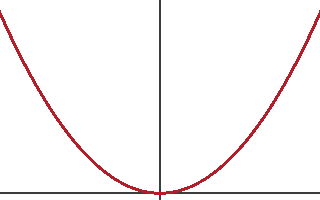
\includegraphics[width=0.6\textwidth]{parabola}
  \caption{The graph of $y = x^2$.}\label{fig:parabola}
\end{figure}

Figure~\ref{fig:parabola} shows a parabola. The code is
\begin{verbatim}
for n in range(10):
    print(n, r(n))   # 100% plain
\end{verbatim}
and, as Hardy wrote,
\begin{quote}
A mathematician, like a painter or a poet, is a maker of patterns.
\end{quote}

\begin{cor}\label{cor:gaps}
$g(x) \ll x^{1/4} \log x$.
\end{cor}

\appendix

\section{A computation}\label{app:comp}

\begin{lemma}\label{lem:numerics}
For $x \le 10^{12}$ we have $g(x) \le 2 x^{1/4}$; Erd\H{o}s and Tur\'an knew this,
see Appendix~\ref{app:comp}.
\end{lemma}

\section*{Acknowledgements}

We thank the referee.

\bibliographystyle{amsplain}
\bibliography{refs}

\end{document}
